% !TEX root = main.tex

%%%%%%%%%%%%%%%%%%%%%%%%%%%%%%%%%%%%%%%%%%%%%%%%%%%%%

\myinput{memory}

%%%%%%%%%%%%%%%%%%%%%%%%%%%%%%%%%%%%%%%%%%%%%%%%%%%%%

\section{Loops}
\label{se:loops}

Loops can easily lead to the path explosion problem: any iteration of a loop can be seen as a {\tt IF-GOTO} statement. Example taken from~\cite{CS-CACM13}:
    \begin{lstlisting}[basicstyle=\ttfamily\small]
    1.  int N = sym_input(); // e.g., read
    2.  while (N > 0) {
    3.    N = sym_input();  
    4.  }
    \end{lstlisting}
The path constraint set of any final state will contain:
  \[ \left ( \bigwedge_{i \in [1, n]]} N_i > 0 \right ) \wedge (N_{n+1} \leq 0) \]
where $N_i$ is the symbol introduced at the i-th iteration.\\

For this reason, it is common to specifically deal with them:
\begin{itemize}

  \item {\em preconditions}: a technique to make it easier to perform symbolic execution on loops is through imposing some preconditions, e.g., use static analysis techniques to understand number of iterations for a loop. See Section~\ref{precontioned-symbolic-execution} for more details.

  \item {\em fixed exploration}: depending on the goal, a symbolic engine may decide to fully explore a loop (e.g., see heuristics presented in~\cite{AEG-NDSS11} and discussed in Section~\ref{heuristics}) or explore only a fixed number of iterations (e.g., up to 3 iterations) in order to avoid path explosion.

  \item {\em approximations}: effects of a loop are often approximated using {\em fixpoints} (e.g., in~\cite{KKM-USEC05,BNS-SP06,CFB-ACSAC06}). A fixpoint F is an approximation of the effect of loop body on an execution state. F approximates the state after the execution of loop whenever the initial state before the loop was F (?). Transforming an execution state to a fixpoint state is defined as widening. Construction of the fixpoint:
  \begin{itemize}
    \item S1: state after first iteration
    \item S2: state after second iteration
    \item compare S1 and S2: assign bottom to each symbol that has been altered
    \item repeat until there is no difference between Si and Si+1
    \item if there is a branch inside the loop, then either the branch is known or its condition is on a symbol which has been assign to bottom. In this case, two parallel states are created and then compared.
  \end{itemize}

\end{itemize}

Notice that detection/analysis of loops can be done using techniques such as~\cite{SGL-TOPLAS96} (e.g., in~\cite{CFB-ACSAC06}).


%%%%%%%%%%%%%%%%%%%%%%%%%%%%%%%%%%%%%%%%%%%%%%%%%%%%%%
\section{Complex objects}

It is common to use {\em lazy initialization} for handling complex memory objects. Notice that if lazy initialization is not used by the symbolic engine, then it is likely that it has to treat complex objects completely symbolically, requiring a constraint solver that is able to solve the resulting constraints. In other words, the solver must support some form of theory of data structures or arrays.

\paragraph{Recursive data structures} Lazy initialization over recursive data structure works~\cite{PV-JSTTT09} as follows:
\begin{itemize}
  \item whenever an instance method is called over a symbolic object, the object is created with uninitialized fields
  \item whenever an uninitialized field of a non-native type is accessed, the symbolic engine non deterministically initialize it with: (a) a {\tt null} reference, (b) a reference to a previously created object, (c) a reference to a new object with uninitialized fields. 
  \item whenever an uninitialized field of a native type\mynote{this is my guess, it's not clear explained in~\cite{PV-JSTTT09}}) is accessed, a new symbolic value is introduced. 
\end{itemize}

\mynote{Merge discussion of {\em lazy initialization} done in Section~\ref{under-constrinained}.}

Notice that if some input preconditions~\ref{precontioned-symbolic-execution} has been set, lazy evaluation should consider and exploit them. For instance, the object may have been marked as acyclic and thus fewer possible alternatives should be considered when initializing a uninitialized field. Further complication~\cite{PV-JSTTT09} may arise for programs that perform destructive updates. 

\paragraph{Input arrays}
It is common that programs may have loops bounded by the length of some input arrays. If this length cannot be statically determined then the symbolic engine may non-deterministically choose when to stop a loop. This means that the number of entries in a symbolic array does not need to be chosen as soon as the symbolic array is created, but this choice can be postponed.

\paragraph{Native code} Several programming languages provide data types that can be very complex. For instance, Java provides the {\tt String} type. Prior works (see, e.g.,~\cite{SHZ-TAIC07}) has presented some approaches for addressing these issues.


%%%%%%%%%%%%%%%%%%%%%%%%%%%%%%%%%%%%%%%%%%%%%%%%%%%%%%
\section{Subroutines and recursion}
\label{se:recursion}


%%%%%%%%%%%%%%%%%%%%%%%%%%%%%%%%%%%%%%%%%%%%%%%%%%%%%%

\myinput{environment}


%%%%%%%%%%%%%%%%%%%%%%%%%%%%%%%%%%%%%%%%%%%%%%%%%%%%%%

\myinput{explosion}

%%%%%%%%%%%%%%%%%%%%%%%%%%%%%%%%%%%%%%%%%%%%%%%%%%
\section{Symbolic executors}

A symbolic execution engine should guarantee three main principles (\cite{MAYHEM-SP12}):
\begin{enumerate}
  \item the system should be able to forward progress for arbitrarily long time, ideally forever, without exceeding the given resources
  \item to maximize performance, no work should be repeated (avoid to restart symbolic / concrete execution)
  \item the system should reuse as much as possible previous analysis results
\end{enumerate}

Based on these principles, symbolic executors can be divided into:

\begin{itemize}
  \item {\em offline} executors (e.g., \cite{SAGE-NDSS08}): one path at time, every run independent from the others, results can be immediately reused, each run restarts the execution of the program from the beginning. In order to perform a run, two inputs must be provided: the target program and a seed input. The program is concretely executed and a trace is recorded. Then the trace is symbolically executed. This can be seen as a form of {\em concolic} execution (see Section~\ref{concolic-execution}).
  \item {\em online} executors (e.g., \cite{KLEE-OSDI08,CKC-TOCS12,AEG-NDSS11}: for each fork, the execution state is cloned. All active execution states are kept in memory, no need to re-execute but huge burden on memory resources. A form of {\em context switch} is often needed. Executors may stop forking at a certain point to allow progress, but then some path are ignored. Memory is saved by aggressive copy-on-write optimization (e.g., immutable state). DFS can be used as exploration strategy in order to minimize memory consumption but can be very slow at doing progress. Notice that since multiple runs may be executed in parallel, isolation must be guaranteed (e.g., keeping different states of the OS by emulating system calls).
  \item {\em hybrid} executors (e.g., \cite{MAYHEM-SP12}): mixed approach. Start with an online approach, if needed switch to offline mode by doing checkpoints. A checkpoint contains the symbolic execution state and replay information. Concrete execution state is discarded since it can be quickly recovered at runtime by using one input generated by the solver before checkpointing.
\end{itemize}


%%%%%%%%%%%%%%%%%%%%%%%%%%%%%%%%%%%%%%%%%%%%%%%%%%%%%%

\myinput{constraints}


%%%%%%%%%%%%%%%%%%%%%%%%%%%%%%%%%%%%%%%%%%%%%%%%%%%%%%
\section{Symbolic execution of binary code}

Symbolic techniques may work on the source code or on the binary code. However, it is not uncommon that both the former and the latter work by reasoning on an intermediate representation of the original code. For instance, ~\cite{KLEE-OSDI08} interprets the LLVM bytecode generated by compiling the source code, while~\cite{ANGR-SP16} reasons on the VEX IR that has been obtained by lifting the binary code.

\begin{figure}[h!]
  \centering
  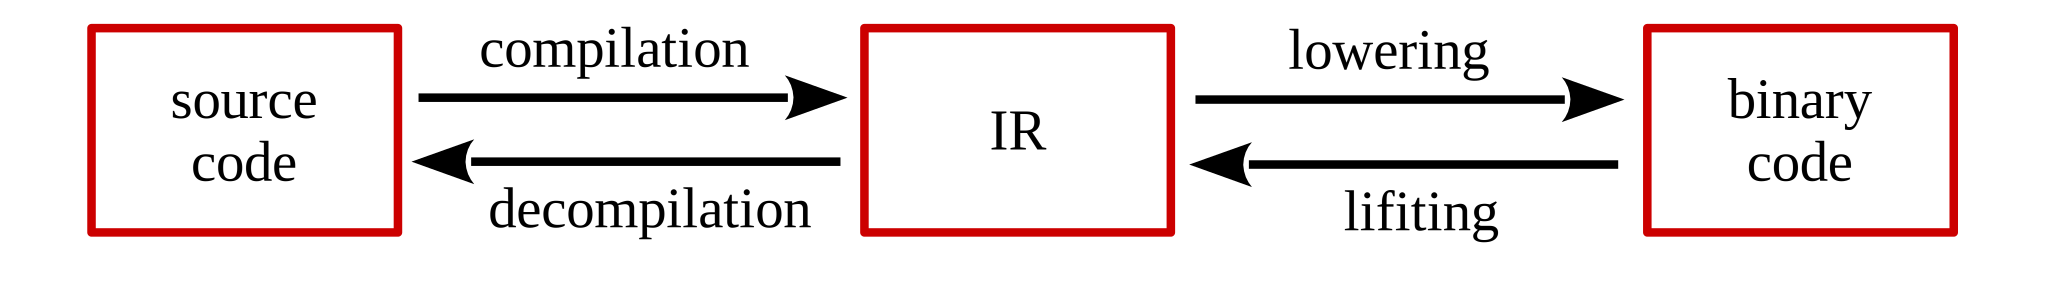
\includegraphics[width=.7\columnwidth]{images/compiler} 
\end{figure}


